\documentclass[aspectratio=169]{beamer}
\mode<presentation>

\usepackage{adjustbox}
\usepackage{relsize}
\usepackage{graphicx}
\usepackage[overlay,absolute]{textpos}

\usepackage{tikz}
\usetikzlibrary{arrows.meta}
\usetikzlibrary{positioning}
\usetikzlibrary{tikzmark}

\graphicspath{{../images}}

\usepackage{fontspec}
\setsansfont{Helvetica Neue Light}[
    BoldFont={Helvetica Neue Bold},
    BoldItalicFont={Helvetica Neue Bold Italic},
    ItalicFont={Helvetica Neue Light Italic}
]
\setmonofont{Iosevka Term}
\newfontface\helvreg{Helvetica Neue}

\title{Stack graphs}
\subtitle{Name resolution at scale}
\author{
    Douglas A. Creager
    \\
    Hendrik van~Antwerpen
}
\institute{
\includegraphics[width=2.5em]{github-mark.pdf}\vspace{2em}}
\date{Eelco Visser Commemorative Symposium\\\textsmaller[1]{April 5, 2023 – TU Delft}}

\setbeamercolor{title}{fg=black}
\setbeamerfont{title}{series=\bfseries,size=\larger[1]}
\setbeamerfont{subtitle}{series=\mdseries,size=\smaller[2]}
\setbeamerfont{author}{size=\smaller[1]}
\setbeamerfont{institute}{size=\normalsize}
\setbeamertemplate{navigation symbols}{}
\setbeamercolor{frametitle}{fg=black}
\setbeamerfont{frametitle}{series=\bfseries}

% Picture credits

\makeatletter
\def\picturecredits{}
\newcommand{\picturecredit}[4]{
    \protected@xappto\picturecredits{
        \textsmaller[3]{Slide \theframenumber} &
        \textsmaller[2]{#1, “#2”} \vspace*{-0.4em} \newline
        \textsmaller[3]{#3, \url{#4}} \\
    }
}
\makeatother

\newlength{\titlewidth}
\newcommand{\flattitle}[3]{
    \settowidth{\titlewidth}{\textbf{\LARGE #3}}
    \begin{textblock*}{\titlewidth}(#1,#2)
        \textbf{\LARGE #3}
    \end{textblock*}
}
\newcommand{\shadowedtitle}[3]{
    \settowidth{\titlewidth}{\textbf{\LARGE #3}}
    \addtolength{\titlewidth}{0.5mm}
    \begin{textblock*}{\titlewidth}(#1+0.4mm,#2+0.4mm)
        \textbf{\LARGE #3}
    \end{textblock*}
    \begin{textblock*}{\titlewidth}(#1,#2)
        \textbf{\textcolor{white}{\LARGE #3}}
    \end{textblock*}
}

\usepackage[outputdir=.build]{minted}
\usemintedstyle{colorful}
\setminted{autogobble,fontsize=\relscale{0.8},frame=single,framesep=6pt,escapeinside=??}

%%%%%%%%%%%%%%%%%%%%%%%%%%%%%%%%%%%%%%%%%%%%%%%%%%%%%%%%%%%%%%%%%%%%%%%%%%%%%%%%
% tikz stuff

\makeatletter
\tikzset{tikzmark suffix=-\theframenumber-\the\beamer@slideinframe}
\makeatother

\tikzset{binding arrow/.style={->, red, thick, -{Triangle[]}}}

\newcommand{\codeline}[3][]{%
    \tikz[remember picture] \draw [overlay, binding arrow, #1] (#2) -- (#3);%
}

\newcommand{\curvecodeline}[4][]{%
    \tikz[remember picture] \draw [overlay, binding arrow, #1] (#2) .. controls #3 .. (#4);%
}

\newcommand{\highlightdef}[1]{%
    \tikz[remember picture]
      \draw [overlay, draw=none, fill=red!25]
        ([xshift=-1pt, yshift=8pt] pic cs:#1_start)
        rectangle
        ([xshift=1pt, yshift=-2pt] pic cs:#1_end)
        ;%
}

\newcommand{\highlightboth}[1]{%
    \tikz[remember picture]
      \draw [overlay, draw=brown, thin, fill=yellow!25]
        ([xshift=-1pt, yshift=8pt] pic cs:#1_start)
        rectangle
        ([xshift=1pt, yshift=-2pt] pic cs:#1_end)
        ;%
}

\newcommand{\highlightref}[1]{%
    \tikz[remember picture]
      \draw [overlay, draw=none, fill=blue!25]
        ([xshift=-1pt, yshift=8pt] pic cs:#1_start)
        rectangle
        ([xshift=1pt, yshift=-2pt] pic cs:#1_end)
        ;
}

%%%%%%%%%%%%%%%%%%%%%%%%%%%%%%%%%%%%%%%%%%%%%%%%%%%%%%%%%%%%%%%%%%%%%%%%%%%%%%%%

\begin{document}

\begin{frame}
    \titlepage
\end{frame}


\section{Code Navigation}

\begin{frame}
    \begin{textblock*}{160mm}(0mm,0mm)
        \picturecredit{Ivan Radic}{Close-up of a compass graffiti on the ground}{CC-BY-2.0}{https://flic.kr/p/2kGKMtM}
        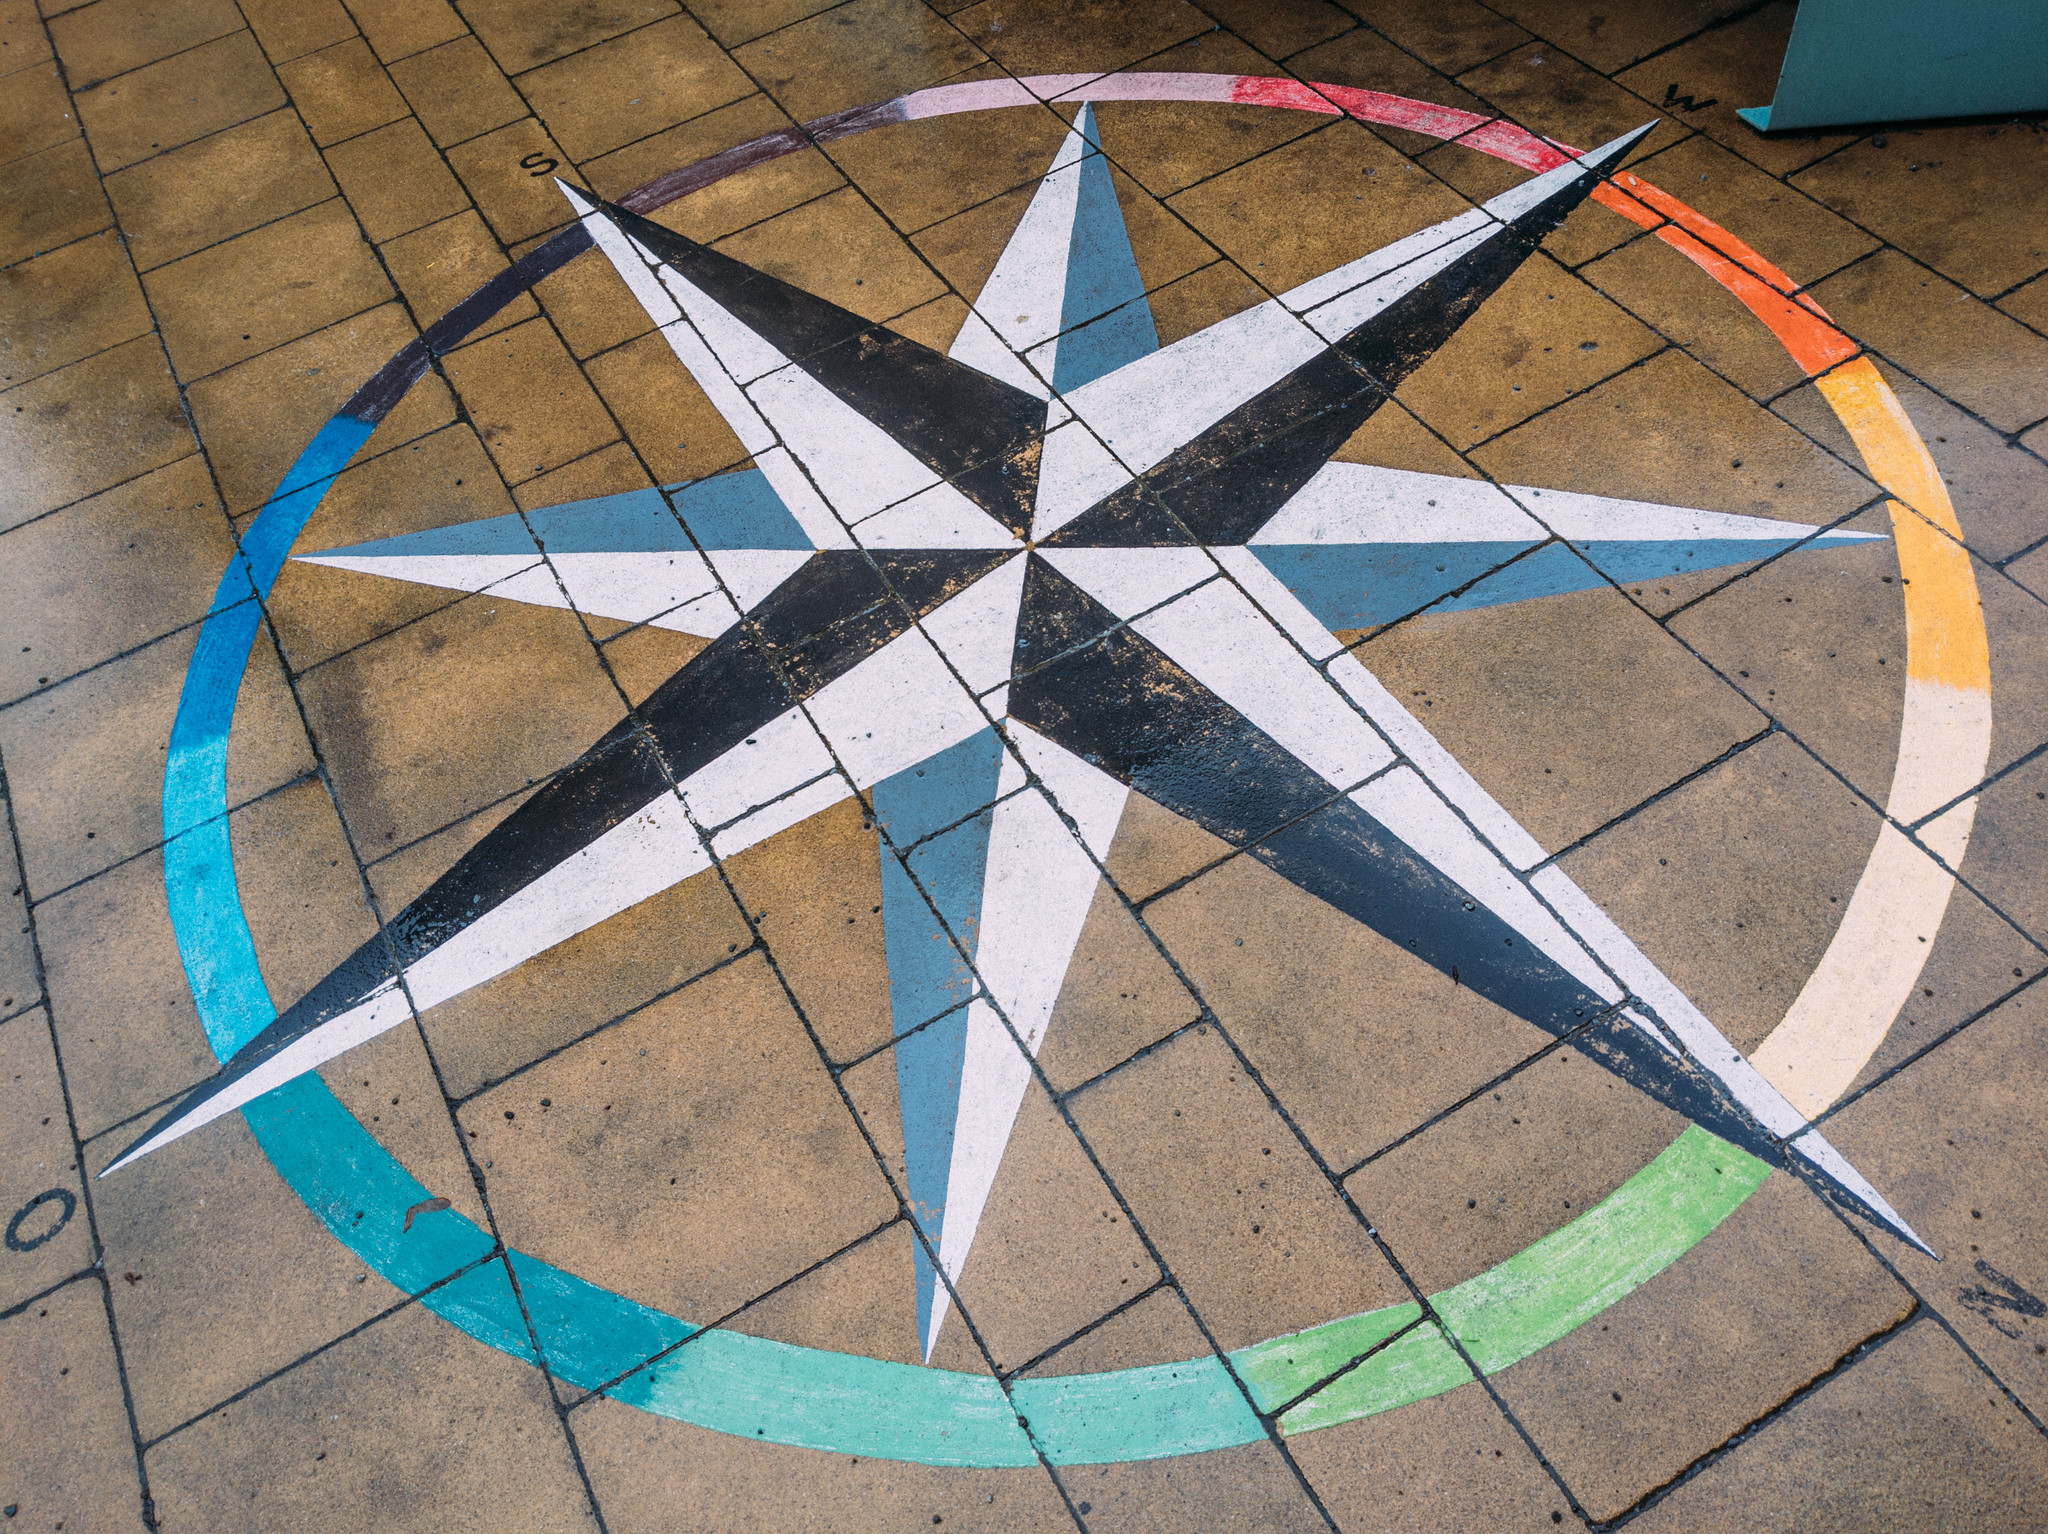
\includegraphics[width=160mm]{compass.jpg}
    \end{textblock*}
    \shadowedtitle{10mm}{10mm}{Code Navigation}
\end{frame}

% easy
\begin{frame}[fragile]
    \frametitle{Code Navigation}
    \highlightdef{def}
    \highlightref{ref}
    \begin{center}
    \begin{minipage}{9em}
    \begin{minted}[label=stove.py]{python}
        def bake():
            pass

        def ?\tikzmark{def_start}?broil?\tikzmark{def_end}?():
            pass

        def saute():
            pass

        ?\tikzmark{ref_start}?broil?\tikzmark{ref_end}?()
    \end{minted}
    \end{minipage}
    \end{center}
    \curvecodeline%
      {[yshift=8pt] pic cs:ref_end}%
      {+(25:2cm) and +(-45:1cm)}%
      {[yshift=-4pt] pic cs:def_end}%
\end{frame}

\begin{frame}
    \begin{textblock*}{160mm}(0mm,0mm)
        \picturecredit{Mustang Joe}{I swear...}{Public domain}{https://flic.kr/p/VSLwD6}
        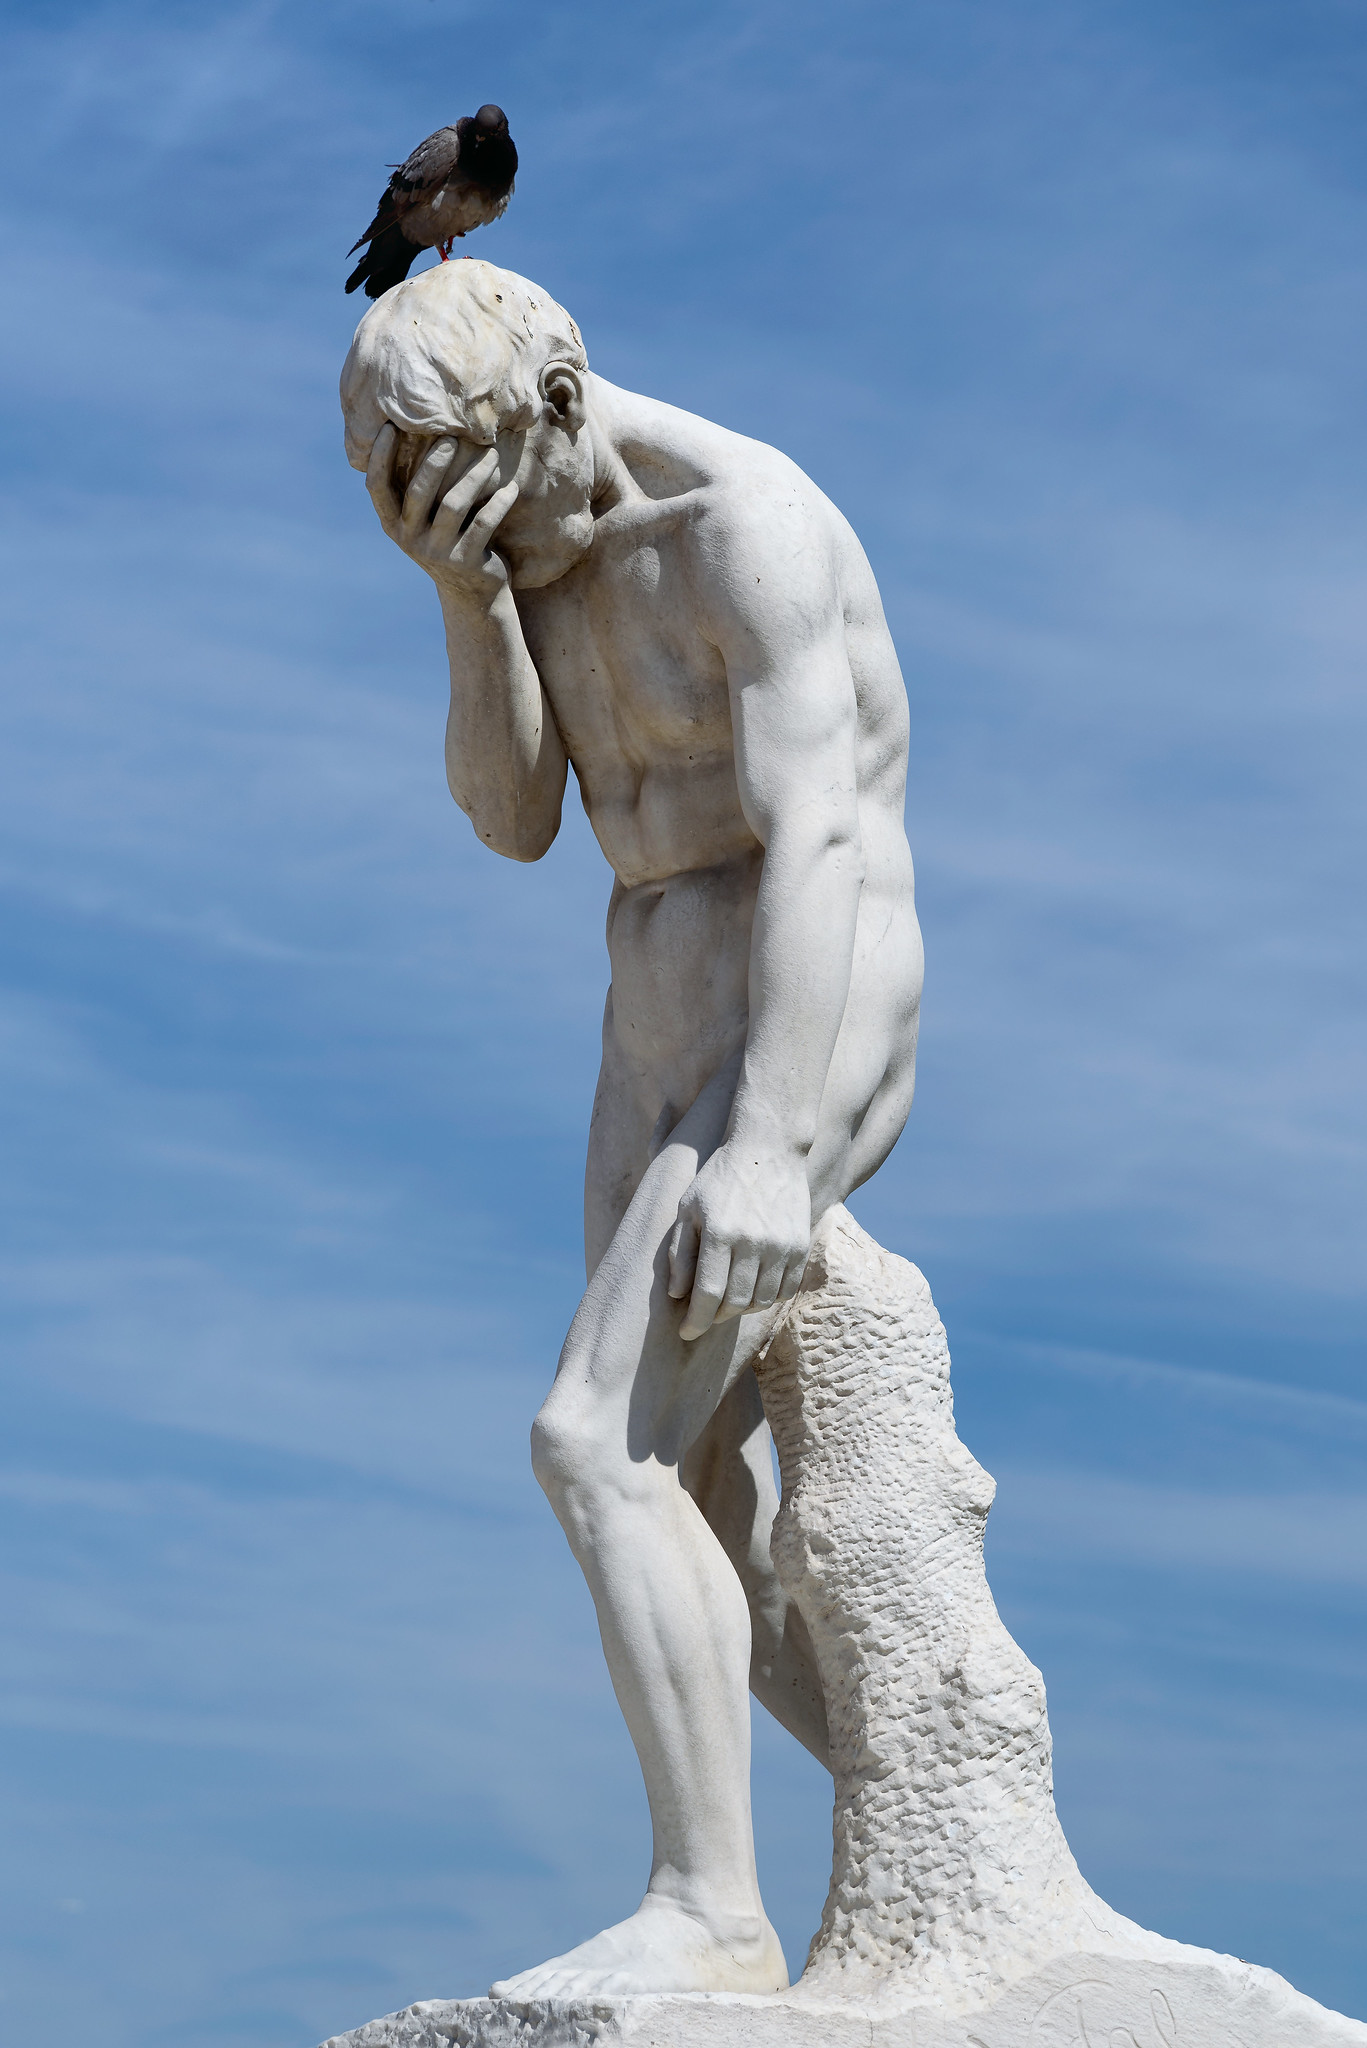
\includegraphics[width=160mm]{facepalm.jpg}
    \end{textblock*}
    \shadowedtitle{140mm - \titlewidth}{25mm}{Why is this hard?}
\end{frame}

% three_files
\begin{frame}[fragile]
    \highlightdef{def}
    \highlightboth{kitchen_import}
    \highlightboth{chef_import}
    \highlightref{ref}
    \frametitle{Multiple files}
    \begin{center}
    \begin{minipage}[t]{22.5em}
    \begin{center}
        
\includegraphics[height=2em]{icons/pan.png}
    \end{center}
    \vskip -1em
    \begin{minipage}[t]{7em}
    \begin{minted}[label=stove.py]{python}
        def bake():
            pass

        def ?\tikzmark{def_start}?broil?\tikzmark{def_end}?():
            pass

        def saute():
            pass
    \end{minted}
    \end{minipage}
    \hspace{0.5em}
    \begin{minipage}[t]{15em}
    \begin{minted}[label=kitchen.py]{python}
        from stove import ?\tikzmark{kitchen_import_start}?*?\tikzmark{kitchen_import_end}?
    \end{minted}
    \end{minipage}
    \end{minipage}
    \hspace{0.5em}
    \begin{minipage}[t]{12em}
    \vskip 8em
    \begin{center}
        
\includegraphics[height=2em]{icons/chef.png}
    \end{center}
    \begin{minted}[label=chef.py]{python}
        from kitchen import ?\tikzmark{chef_import_start}?broil?\tikzmark{chef_import_end}?

        ?\tikzmark{ref_start}?broil?\tikzmark{ref_end}?()
    \end{minted}
    \end{minipage}
    \end{center}
    \curvecodeline%
      [-]%
      {[yshift=10pt] pic cs:ref_end}%
      {+(45:1cm) and +(-155:1cm)}%
      {[yshift=-4pt] pic cs:chef_import_start}%
    \curvecodeline%
      [-]%
      {[xshift=10pt, yshift=10pt] pic cs:chef_import_start}%
      {+(90:5cm) and +(75:2cm)}%
      {[xshift=4pt, yshift=10pt] pic cs:kitchen_import_start}%
    \curvecodeline%
      {[xshift=1pt, yshift=-4pt] pic cs:kitchen_import_start}%
      {+(-105:1cm) and +(75:1cm)}%
      {[xshift=-6pt, yshift=10pt] pic cs:def_end}%
\end{frame}

% three_files_updated
\begin{frame}[fragile]
    \frametitle{Code changes over time}
    \highlightdef{def1}
    \highlightdef{def2}
    \highlightboth{import}
    \highlightref{ref}
    \begin{center}
    \begin{minipage}[t]{22.5em}
    \begin{center}
        
\includegraphics[height=2em]{icons/pan.png}
    \end{center}
    \vskip -1em
    \begin{minipage}[t]{7em}
    \begin{minted}[label=stove.py]{python}
        def bake():
            pass

        def ?\tikzmark{def1_start}?broil?\tikzmark{def1_end}?():
            pass

        def saute():
            pass
    \end{minted}
    \end{minipage}
    \hspace{0.5em}
    \begin{minipage}[t]{15em}
    \begin{minted}[label=kitchen.py]{python}
        from stove import *

        def ?\tikzmark{def2_start}?broil?\tikzmark{def2_end}?():
            print("We're broiling!")
            import stove
            return stove.broil()
    \end{minted}
    \end{minipage}
    \end{minipage}
    \hspace{0.5em}
    \begin{minipage}[t]{12em}
    \vskip 8em
    \begin{center}
        
\includegraphics[height=2em]{icons/chef.png}
    \end{center}
    \begin{minted}[label=chef.py]{python}
        from kitchen import ?\tikzmark{import_start}?broil?\tikzmark{import_end}?

        ?\tikzmark{ref_start}?broil?\tikzmark{ref_end}?()
    \end{minted}
    \end{minipage}
    \end{center}
    \curvecodeline%
      [-]%
      {[yshift=10pt] pic cs:ref_end}%
      {+(45:1cm) and +(-155:1cm)}%
      {[yshift=-4pt] pic cs:import_start}%
    \curvecodeline%
      {[xshift=10pt, yshift=10pt] pic cs:import_start}%
      {+(90:5cm) and +(75:2cm)}%
      {[xshift=-6pt, yshift=10pt] pic cs:def2_end}%
\end{frame}

% python_class
\begin{frame}[fragile]
    \frametitle{Type-dependent name resolution}
    \begin{center}
    \highlightdef{def}
    \highlightref{ref}
    \begin{minipage}[t]{25.5em}
    \begin{center}
        
\includegraphics[height=2em]{icons/pan.png}
    \end{center}
    \vskip -1em
    \begin{minipage}[t]{10em}
    \begin{minted}[label=stove.py]{python}
        class?\tikzmark{class}? Stove?\tikzmark{class_def}?(object):
            def bake(self):
                pass

            def ?\tikzmark{def_start}?broil?\tikzmark{def_end}?(self):
                pass

            def saute(self):
                pass
    \end{minted}
    \end{minipage}
    \hspace{0.5em}
    \begin{minipage}[t]{15em}
    \begin{minted}[label=kitchen.py]{python}
        from stove import ?\tikzmark{kitchen_import}?*
    \end{minted}
    \end{minipage}
    \end{minipage}
    \hspace{-5.5em}
    \begin{minipage}[t]{12em}
    \vskip 6em
    \begin{center}
        
\includegraphics[height=2em]{icons/chef.png}
    \end{center}
    \begin{minted}[label=chef.py]{python}
        from kitchen import ?\tikzmark{chef_import}?Stove

        stove?\tikzmark{instance_def}? = Stove?\tikzmark{class_ref}?()
        stove?\tikzmark{instance_ref}?.?\tikzmark{ref_start}?broil?\tikzmark{ref_end}?()
    \end{minted}
    \end{minipage}
    \end{center}
    \curvecodeline%
      [-]%
      {[xshift=-10pt, yshift=-3pt] pic cs:ref_end}%
      {+(-135:0.2cm) and +(-45:0.2cm)}%
      {[xshift=-10pt, yshift=-3pt] pic cs:instance_ref}%
    \curvecodeline%
      [-]%
      {[xshift=-23pt, yshift=2pt] pic cs:instance_ref}%
      {+(180:0.2cm) and +(180:0.2cm)}%
      {[xshift=-23pt, yshift=2pt] pic cs:instance_def}%
    \curvecodeline%
      [-]%
      {[xshift=-10pt, yshift=8pt] pic cs:instance_def}%
      {+(65:0.3cm) and +(115:0.3cm)}%
      {[xshift=-10pt, yshift=8pt] pic cs:class_ref}%
    \curvecodeline%
      [-]%
      {[xshift=-4pt, yshift=-3pt] pic cs:class_ref}%
      {+(-35:0.5cm) and +(-90:1cm)}%
      {[xshift=10pt, yshift=-3pt] pic cs:chef_import}%
    \curvecodeline%
      [-]%
      {[xshift=10pt, yshift=10pt] pic cs:chef_import}%
      {+(90:3cm) and +(-90:1cm)}%
      {[xshift=2pt, yshift=-3pt] pic cs:kitchen_import}%
    \curvecodeline%
      [-]%
      {[xshift=2pt, yshift=10pt] pic cs:kitchen_import}%
      {+(90:2cm) and +(90:2cm)}%
      {[xshift=-10pt, yshift=8pt] pic cs:class_def}%
    \curvecodeline%
      [-]%
      {[xshift=-6pt, yshift=-2pt] pic cs:class_def}%
      {+(-45:2cm) and +(90:2cm)}%
      {[xshift=4pt, yshift=10pt] pic cs:class_ref}%
    \curvecodeline%
      [-]%
      {[xshift=4pt, yshift=-3pt] pic cs:class_ref}%
      {+(-90:2.5cm) and +(-90:6.5cm)}%
      {[xshift=-10pt, yshift=-2pt] pic cs:class}%
    \curvecodeline%
      {[xshift=-10pt, yshift=8pt] pic cs:class}%
      {+(75:1cm) and +(115:1cm)}%
      {[xshift=-10pt, yshift=6pt] pic cs:def_end}%
\end{frame}


\begin{frame}
    \begin{textblock*}{160mm}(0mm,0mm)
        \only<1>{
            \picturecredit{Mark Gunn}{This just tern'ed into a swarm!}{CC-BY-2.0}{https://flic.kr/p/P11JH1}
            \adjincludegraphics[Trim=0 0 0 1.5in, width=160mm]{terns.jpg}
        }
    \end{textblock*}
    \begin{textblock*}{80mm}(80mm,0mm)
        \only<2>{\adjincludegraphics[Trim=0 0 0 1.5in, width=160mm, Clip={0.5\width} 0 0 0]{terns.jpg}}
    \end{textblock*}

    \begin{onlyenv}<2>
    \frametitle{SCALE}
    200 million repositories and counting
    \vskip 1em
    2 billion contributions \\
    in the last 12 months
    \vskip 1em
    500 programming languages
    \end{onlyenv}
\end{frame}


\begin{frame}
    \begin{textblock*}{160mm}(0mm,-15mm)
        \picturecredit{Katja Schulz}{Inchworm}{CC-BY-2.0}{https://flic.kr/p/PJMP4w}
        \adjincludegraphics[width=160mm]{inchworm.jpg}
    \end{textblock*}
    \shadowedtitle{26mm}{5mm}{Incremental processing}
\end{frame}


\begin{frame}[t]
    \frametitle{Picture credits}
    \begin{tabular}{lp{0.75\textwidth}}
    \picturecredits
    \end{tabular}
\end{frame}


\end{document}
